\documentclass[12pt]{article}
\usepackage{candor, setspace}
\usepackage[verbose]{wrapfig}
\hyphenation{frame-shifts}

\newcommand{\BWFtitle}[1]{A Computational Modeling for Translational
  Efficiency and Frameshifts in #1{Escherichia coli} Using Genetic Signal
  Processing}
\newcommand{\BWFauthors}{Hao Lian, Vivek Bhattacharya, and Daniel
  R. Vitek}

\usepackage[final, colorlinks=true, linkcolor=BWFBlue,
  citecolor=BWFGreen, urlcolor=BWFRed, pdftitle={\BWFtitle{}},
  pdfauthor={\BWFauthors}, pdfsubject={Genetics}, pdfcreator={The
    Frameshift Kids}, pdfkeywords={bioinformatics,
    genetics,biology,frameshifts,ecoli,prfB,rpoS,bGH,ecoli,translation},
  pdfstartview={FitH}, backref]{hyperref}

\linespread 2

\usepackage{titlesec}
\titleformat{\section}{\bfseries}{\thesection.}{.5em}{\MakeUppercase}
\titleformat{\subsection}{\bfseries}{\thesubsection.}{.5em}{\normalsize}
\titlespacing{\section}{0pt}{0.5\baselineskip}{*0}
\titlespacing{\subsection}{0pt}{0.5\baselineskip}{*0}
\titlespacing{\subsubsection}{0pt}{0.5\baselineskip}{*0}

\author{\sc{\BWFauthors}}
\date{{\sc \today}}
\title{\bf{\BWFtitle{\emph}}}

\begin{document}
% Title, table of contents, and abstract start things off.
\pagenumbering{roman}
\begin{singlespace}
  \maketitle
  \tableofcontents
\end{singlespace}

\clearpage
\begin{center}
\end{center}
\begin{abstract}\begin{normalsize}
  \textbf{``\BWFtitle{\emph}''}
  
  In modern genetics, \ecoli\ is used as an expression system to commercially
  produce proteins.  However, sequence-dependent
  features, such as rare codons and codon bias, have large effects on translational
  efficiency.  To tackle this problem, we proposed a stochastic model to computationally estimate
  translational efficiency and predict frameshifting, uniting ideas from biological literature.
  We propose two metrics that bear considerable predictive power toward translational efficiency.
  We then test our model on a large sample of sequences from the \ecoli\ genome and
  found over 90\% of them have predicted high yields, which correlates
  result that concurs with biological knowledge.  Moreover, it predicts ribosomal proteins
  to translate at even more efficient rates, also experimentally verified.
  Computational results also concur with experiments conducted on translational
  rates of recombinant bovine growth hormone sequences and variations of \prfB, a gene
  with a programmed frameshift. Various explanations for outliers, such as protein-ribosome
  interactions, are discussed. We then test of our model's predictive
  power, a work in progress.  With more data, this model provides
  promise to serve as a quick, computation means to predict the
  translational behavior of recombinant proteins in \ecoli.
\end{normalsize}\end{abstract}  
  
\clearpage
\pagenumbering{arabic}

\section{Purpose}
We are part of an ongoing research project
investigating the application of bioinformatics
and genetic signal processing to better understand how
information is encoded and decoded from nucleic acids.  The particular
focus of the current research ribosomal translation within
bacteria.  Previous researchers~\cite{lalit:mechanics}
have developed a deterministic model
of the translational reading frame by studying the
programmed frameshift present in the prfB gene of \ecoli.  The focus
of our studies was to improve the model and apply its vatic powers.

\section{Rationale}
\citet{kozak05} and \citet{kane95} studied the impact
of sequence-dependent features, especially with regard to codon bias 
and rare codon usage, on translational efficiency.  The importance of 
relationship is even more pronounced in recombinant 
proteins~\cite{sorensen05}.  In addition, secondary structure problems 
during protein folding can decrease translational 
efficiency~\cite{kozak05}.  However, scientists do not fully
understand the specific connections between efficiency and these
sequence-dependent factors, as even eliminating troublesome factors
does not always increase efficiency. The goal of our studies is to
advance the development of a computational method that can increase
translational efficiency through mRNA sequence modifications. If
successful, this work streamlines gene sequence optimization in the
production of high-yield, recombinant proteins. Creating cell lines
that synthesize commercially viable yields in fields ranging from
medicine to agriculture is a significant challenge that our model
addresses. In addition, a successful model implies a mechanism by
which molecular biologists can test the stable maintenance of
elongation.

Earlier, \citet{lalit:jbsb} created a deterministic model of
frameshifting based on the hybridization between the 16S rRNA tail and
upstream mRNA nucleotides.  The periodicity of this
signal~\cite{lalit:jbsb} suggests that the force emerges from the free
energy during hybridization acts as a correcting mechanism,
stabilizing codon choice.  In this manner, early errors in the reading
frame are rarely propagated.  Some limitations of the deterministic 
model are discussed in \autoref{stochastic}.

Because the ribosome's displacement from the zero reading frame is
almost always nonzero, we create a new metric of efficiency: the total 
deviation from the intended reading frame.  This metric
(\autoref{section:deviation}) then roughly correlates to translational
efficiency.  Throughout this paper, we use this and other metrics to
optimize tRNA availabilities in order to distinguish between
high-efficiency and low-efficiency sequences. We also use our new
metric to optimize the efficiency of a translationally regulated gene, 
and apply our new metric to ribosomal proteins and the entire \ecoli\ 
genome to see if the model is robust over many genes.

\section{Prior Model}
\subsection{Free Energy}
\label{freeenergy}

Hybridization between two RNA sequences changes the free energy in a cell.
Such hybridization occurs between the small
ribosomal subunits---especially the 16s rRNA tail---the mRNA, and the tRNA~\cite{starmer}.
\citet{sd} observed that the $3'$ end of the 16S rRNA is complementary to a sequence found 
directly upstream of many prokaryotic mRNAs; they hypothesized that RNA hybridization 
plays an important role in translation initiation, later
experimentally confirmed~\cite{hui,jacob}.

\citet{weiss87} subsequently observed that changes in the 16S tail can 
significantly change the frequency of frameshifting in \prfB, an \ecoli\ gene 
known to frameshift at the 25$^\textrm{th}$ codon.  These results suggest that 
the 16S tail is positioned to interact with the mRNA during translation elongation. 
\citet{xray} supported the spatial accessibility of the 16S tail with the mRNA with 
X-ray crystallography data.

\citet{freier} proposed a thermodynamic model for calculation of free energy values,
modeling the hybridization of permutations of RNA \emph{doublets}, pairs of consecutive nucleotides.

\subsection{Deterministic Model}
\citet{lalit:mechanics} assumed a sinusoidal model 
(and verified it with a fast Fourier transform) for
free energy that projects free energy onto magnitude and
phase through a memory model that stores three values
in a phasor, a concept from physics. Then,
they visualize free energy from polar plots where frameshifts
occur along defined boundaries for a given species.

% Looks almost sinusoidal as you move the codon across; good fit
 
\citeauthor{lalit:mechanics} then represent the cumulative energy phasor
at codon $k$ as $\bvec{V} = Me^{i\theta}$, where $i$ is the imaginary
constant, from which they calculate the magnitude and phase, modeled
on a polar plot, via
trigonometry. Differentiating the energy phasor
with respect to distance along the mRNA strand gives 
vector $\bvec{D}$, the force~\cite{lalit:mechanics}
that acts on the ribosome that keeps the mRNA in the reading frame.
 
The time that the force acts on the ribosome depends upon
the tRNA availability associated with the codon at the A-site 
and interactions between said tRNA and the ribosome. [Dr. Stomp, references please!]
\citeauthor{lalit:mechanics} represent this with a deterministic model: For each codon,
a number of ``wait cycles," a function of the rarity of the
tRNA, correspond to time the force can
increment displacement from the current reading frame.  In the
deterministic model, the force acts for \emph{exactly} the number
of cycles given a codon. \cite{lalit:mechanics}'s model then simulates hybridization between the
16S ribosomal subunit and a given mRNA strand: First, the 13-base 16S
tail of \ecoli\ hybridizes with the first 13 bases of a sequence,
which includes a 12-base leader sequence, to determine the free energy 
value of the first amino acid. The algorithm then similarly calculates
the free energy for the entire sequence~\cite{starmer}.

\subsection{Frameshifts}
\label{section:frameshifts}

\begin{cfigure}
  \caption{Plots of~\prfB}
  \label{prfB:detplots}
  \subfloat[Deterministic displacement]{
    \label{prfB:deterministic:sub}
    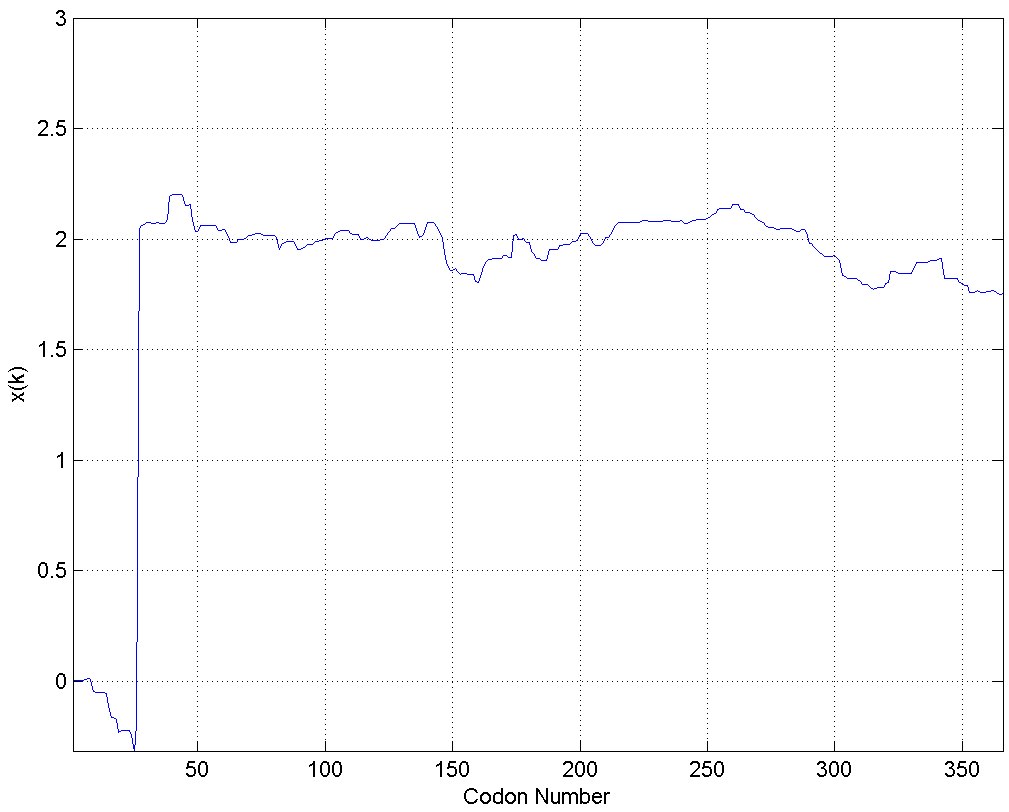
\includegraphics[width=0.5\textwidth]{prfB/deterministic}
  }
  \subfloat[Polar plot]{
    \label{prfB:polar:sub}
    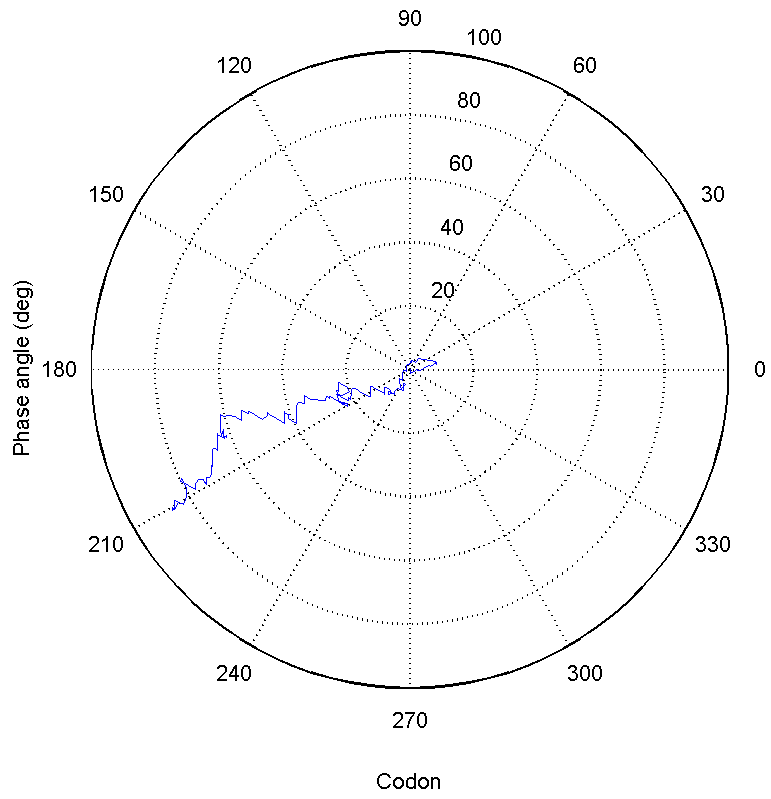
\includegraphics[width=0.4\textwidth]{prfB/polar}
  }
\end{cfigure}

First, \citeauthor{lalit:mechanics} let a displacement of $x = 0$ correspond
to the zero reading frame and increments of \emph{two} to represent a
one-nucleotide change. For example, $x =2$ represents the +1 frame.
They prove that both $x = 0$ and $x = 2$ are fixed
(stable) points in displacement in their model, as expected.

% bitzer 5.3, b/c near 0, p(indecision) is large -- > spends more time  

A jump from approximately $x = 0$ to $x = 2$ in a span of only
base pair is then the first indication of a $+1$ frameshift; it
suggests the ribosome skips one entire base pair in the mRNA sequence.
\autoref{prfB:deterministic:sub} shows the displacement plot per this
deterministic model for \prfB, a gene with a unique programmed $+1$
frameshift, which exists at codon 25. In conjunction with this
characteristic plot, a $+1$ frameshift also displays an equally
characteristic clockwise 120\degree\ phase angle rotation from the
species angle, the average phase of the free energy signals of a
number of verified \ecoli\ genes that stay in frame
\cite{lalit:mechanics}.  We interpret the free energy signal's
alignment with the sudden jump in displacement as a sustained
frameshift because the physics then indicate a stable shift in
reading frame. Since the free energy signal has a period of one
codon~\cite{lalit:mechanics}, a $+1$ frameshift the free energy signal
must undergo a phase shift of one-third of an entire period
(\autoref{prfB:polar:sub}).

\section{Computational Methods}

\subsection{Stochastic Displacement Model}
\label{stochastic}

As mentioned, the gene \prfB\ exhibits a programmed frameshift under
the deterministic model by jumping in displacement to $x=2$.  Certain
genes, however, demonstrate equivocal, ambiguous behavior near
$x = \pm 1$~\cite{lalit:mechanics}.  In the deterministic model, we lack the
sensitivity needed to clearly discern a programmed
frameshift. Worse, the model may not show these unstable
behaviors at all. The nondeterministic
behavior of translation and the presence of noise limits the model's
ability to better model it. Therefore, we retooled the model to be
stochastic the incorporation of sinusoidal probability.\footnote{
  The model, written in Perl and Matlab, is available online with
  documentation, algorithms, and additional tools.
}

At each wait-cycle in elongation, we propose the ribosome makes a
decision: stay in the current reading
frame, move to the $\pm 1$ reading frames, or proceed to the next cycle.
In addition, because the 
number of wait cycles is inversely proportional to the tRNA availability of 
the codon in the current reading frame (the A-site), rarer codons force the 
ribosome to wait longer for the appropriate
aa-tRNA. \citet{lalit:mechanics}, in turn, calculated tRNA
availability values from existing research~\cite{ikemura} that
indicates a relationship between it and codon frequency. From this
body of work, we later created a different algorithm to
calculate tRNA availabilities (\autoref{section:parameters}).

Let $abcd$ be a sequence of four nucleotides, with $abc$ in the
current and $bcd$ in the +1 reading frame, and let $x$ be the
displacement of the current wait cycle of the ribosome.  As the
incremental displacement approaches +1, the probability of choosing
codon $bcd$ increases and the probability of choosing codon
$abc$ decreases.

We model this behavior using even powers of
cosine and sine functions for $abc$ and $bcd$, defining
$\omega$ as the \emph{weight} that is directly proportional to
the probability.
\begin{equation}
  \omega_{abc} = \cos^{10}{\frac{x\pi}{4}} \text{ and } \omega_{bcd} =
  \sin^{10}{\frac{x\pi}{4}}.
  % Foonote
  \footnote{The cosine and sine functions are taken to the tenth power
    here. These parameters can change.}
\end{equation}
If the ribosome lies completely and thus is stable in the
zero frame, then the probability
of staying in that frame is one.  Consequently, a ribosome
fully in the +1 frame ($x=2$) has no chance of going to the zero
frame, hence the requirement for a period of two base pairs ($x=4$) in
these functions.

Suppose we are on a wait cycle at codon $abc$ with $N_{abc}$ total
cycles allocated. Let $P$ be the instantaneous probability of staying
in the current reading frame at the next move, which we know is
proportional to the weight (above) $\omega_{abc}$. Let $1/n_{abc}$ be
the constant of proportionality, implying $n =
\omega_{abc}/P$.\footnote{
  We can derive $n$ as follows: Suppose the ribosome is at
  the zero frame exactly without any force pushing it. Then $\omega =
  cos^{10}(0) = 1$, implying $P = 1/n$. Assume the probability of
  moving (1/2) is just as likely as the probability of not moving
  (1/2). Suppose there are $N$ wait cycles. Then $1 - (1 - \omega/n)^N
  = 1/2$, implying $n = \sqrt[N]{2}/(\sqrt[N]{2} - 1)$. We also have
  $\lim_{N\rightarrow\infty}(n) = N/\ln{2}$. Thus, the
  probability of choosing a codon at a cycle is proportional to its
  TAV because $N$ is proportional to its TAV, which coincides with intuition.
}
Then the aggregate probability of choosing codon $abc$ after $K$ cycles is
the probability of not failing to change the reading frame ($1 - P$)
at every cycle for $K$ cycles. Hence, 
\begin{equation}
  1 - \prod_{i=1}^K \left( 1 - \frac{\omega_i}{n} \right) \text{ where }
  \omega_i = \cos^{10}{\frac{x_i\pi}{4}},
  % Footnote
  \footnote{The weight, of
    course, depends upon the frame choice in question.}
\end{equation}

\subsection{Consequences of the Stochastic Model}
The stochastic model introduced a new concept into the model proposed by
\citet{lalit:mechanics}: The ribosome has a finite probability of
``choosing the wrong codon," in
essence accepting the tRNA of an out-of-frame, due to a high availability
of the tRNA or a more applicable shape. This is definitely not a programmed frameshift
frameshift, which is when the force pushes the ribosome to an unstable
point and moves it quickly to the +1 reading frame to regain stability.
Programmed frameshifts take place over the span of just
one codon; the graph never approaches $x=2$ over multiple codons.

An incorrect codon choice can occur when displacement nears $x = \pm 1$.
At this point, both the 0 and the +1 reading frame have a finite
probability of occupying the A-site in the ribosome. From the probability
equations, the ribosome increasingly tends to stabilize around
the +1 frame by accident.  Unlike a frameshift, this results from
the slow digression from the true alignment and occurs over a number of codons.
As the ribosome nears $x = 1$, the values for both the sine 
and cosine functions drop, thus increasing the chance of increasing
the time required for translation. This models the physical
behavior of ribosome's tendency to pause as it stabilizes upon an aa-tRNA in the A-site.

Choosing the wrong codon is a purely stochastic phenomenon; only through our new
model can we actually track the actions of the ribosome throughout the course
of translation.  Due to a general experimental conceptualization of the physics involved,
as described above, we believe that the stochastic model has the potential to 
measure translational efficiency.

\section{Analysis}
To test our computational model, we ran a number of
experiments to analyze sequences present in the \ecoli\ genome.

\subsection{Measures}
\label{section:metrics}

As this model is stochastic, multiple runs (the sample size) of the same sequence must be analyzed.
As such, we propose two metrics for analysis of a number of different runs 
simultaneously. 

\subsubsection{Error-Free Rate}
\label{section:efr}
When studying a
sequence with a programmed frameshift, \emph{error-free rate} measures the percentage of runs 
during which the ribosome chooses the correct codon
at \emph{every} juncture.  For a +1 frameshift, the ribosome must
choose the +1 frame at the frameshift codon and stay in the 0 frame before
and the +1 frame after in order for the run to be a success.

\subsubsection{Displacement Deviation}
\label{section:deviation}

We define \emph{displacement deviation} to be
\begin{equation}
    d = \sqrt{\frac{\sum_i (x_i - \beta_i)^2}{N}},
\end{equation}
where $\beta_i$ is the predicted reading frame at codon $i$, $x$ is
the displacement at codon $i$, and $N$ is the total number of codons
as a measure of the deviation of the sequence from the expected
reading frame.  Usually $\beta_i = 0$ unless a programmed frameshift
exists as it does for \prfB.  For example, for \prfB\ $\beta_i = 2$
for all $i \geq 25$ because \prfB\ frameshifts at codon 25
\textsc{uga} and the model represents a frameshift with +2
displacement per \autoref{section:frameshifts}.

\subsection{\prfB\ and Related Sequences}
In the first test of our model, we investigated the gene
\prfB\footnote{\prfB\ encodes protein release factor 2, which enters
  the A-site and cause protein synthesis to terminate at the stop
  codons \textsc{UGA} and \textsc{UAA}, which allows it to regulate
  its own production.}, which has a programmed frameshift.
We downloaded the nucleotide sequence for \prfB\ from
NCBI's Genbank database.\footnote{\url{http://www.ncbi.nlm.nih.gov/},
  accession number: NC\_000913, \prfB}

\citet{weiss87} conducted a number of experiments regarding
\prfB\ to test how mutations in the sequence affects the rate of
frameshifting.  They present a total of 35 sequences in their paper,
along with measures of translational efficiency.  Running all of
them and correlating with their error-free rates, we hypothesize that
genes found to frameshift at high rates by
\citeauthor{weiss87} should also show high error-free rates under
our model.

\subsection{The \ecoli\ Genome and Ribosomal Proteins}
Our model also addresses
translational efficiency. We hypothesize that displacement deviation
provides a suitable metric for translational efficiency: A lower
deviation would correspond to a more efficient sequence.

We base this hypothesis on the idea that if, at each wait cycle, the
ribosome fails to stabilize in a period of indecision, the probability
that it will change reading frames increases. The translational
process resolves this indecision either by stabilizing around the
incorrect +1 or -1 reading frame or pausing. The former synthesizes an
incorrect primary structure or causes premature truncation due to an
out-of-frame stop codon while the latter preserves fidelity at the
expense of speed. That is, while a single run may produce
a working primary structure of the protein, the gene in question
ultimately is less efficient than a synonymous gene with lower
aggregate probabilities, whether we express the aggregate measure as the
error-free rate (\autoref{section:efr}) or displacement deviation
(\autoref{section:deviation}). In addition, a greater deviation from
the zero axis inherently implies a longer time for translation, 
since proximity to $\pm1$ would increase the probability of not choosing
either codon, i.e., waiting. A high value thus reduces translational
efficiency, again contributing to the aggregate probability of
translational failure.

To this end, we performed two tests. In one test, we ran the model on
all the 4364 genes provided by the Ecogene database of
\ecoli\ genes\footnote{\url{http://ecogene.org/}}, selected for the
database's reliability. We predict the majority exhibit low
displacement deviations from the inherent tendency of evolution toward
high gene stability and thus high translational efficiency. In another
test, we looked at ribosomal proteins, known to have high levels of
expression~\cite{rpoS:process}. There we predict lower, on average,
deviation than those of the \ecoli\ gene sample.
	
\subsection{Bovine Growth Hormone}
Our final test involved the analysis a set of sequences known to 
be translationally regulated.  \citet{schoner:bgh} created a set 
of eight sequences in an empirical effort to increase the yield 
of recombinant bovine growth hormone (bGH) synthesized in an 
\ecoli\ expression system. \citeauthor{schoner:bgh} noted that 
these sequences are, in fact, translationally regulated, 
presenting a set of eight sequences, four of which are expressed 
at significantly higher levels than the others. We predict that 
the sequences that are highly expressed in \ecoli\ should have 
lower displacement deviations.

\subsection{Parameters}
\label{section:parameters}
For all computational experiments in this report, we use a species
angle of $\theta_{\rm{sp}} = -30\degree$ and an initial displacement of 0.1,
in accordance with \citet{lalit:mechanics} and experimentation.
Later in this report, we explore
the effects of changing the species angle and initial displacement on the
error-free rate of \prfB.

A parameter that is much more difficult to estimate
is tRNA availability value (TAV).
\citeauthor{lalit:mechanics} base the tRNA availability values on codon usage, 
surveying genes from \ecoli.
Although this assumption has experimental basis~\cite{ikemura}, 
it is possible that the true values for these numbers may differ.
We chose to calibrate TAV vectors from existing experimental data, 
designing a genetic algorithm to improve these values based on 
the bovine growth hormone (bGH) sequences while remaining close 
to the values \citeauthor{lalit:mechanics} determined.

We optimize the separation between the displacement deviations of the 
high-yield and low-yield sequences. First, we generate a list of 
randomly modified TAV vectors and calculate the ratio of the 
displacement deviation (\autoref{section:deviation}) for the four 
high-yield sequences to that of the other four. From there, we sort the 
modified TAV vectors by to this ratio and discard the worst half of the 
vectors. We then choose two of the remaining vectors, with the chance 
of each vector being proportional to its rank.  We then take a weighted 
average of the two vectors and spawn a new vector.  After creating the 
next generation according to a constant ``gene pool'' size, we delete 
the previous generation  and repeat. After a fixed number of 
generations, the algorithm terminates and returns the optimal TAV vector.

This algorithm did not significantly alter the TAV vectors; the average 
change to each value in the vector was merely 15.99\%.  The new values
are used throughout the paper.

\section{Results}
\subsection{\prfB}

\begin{cfigure}
  \caption{Plots of \prfB\ in a stochastic model}
  \label{prfB:stochplots}
  \subfloat[Displacement Plot]{
    \label{prfB:disp:sub}
    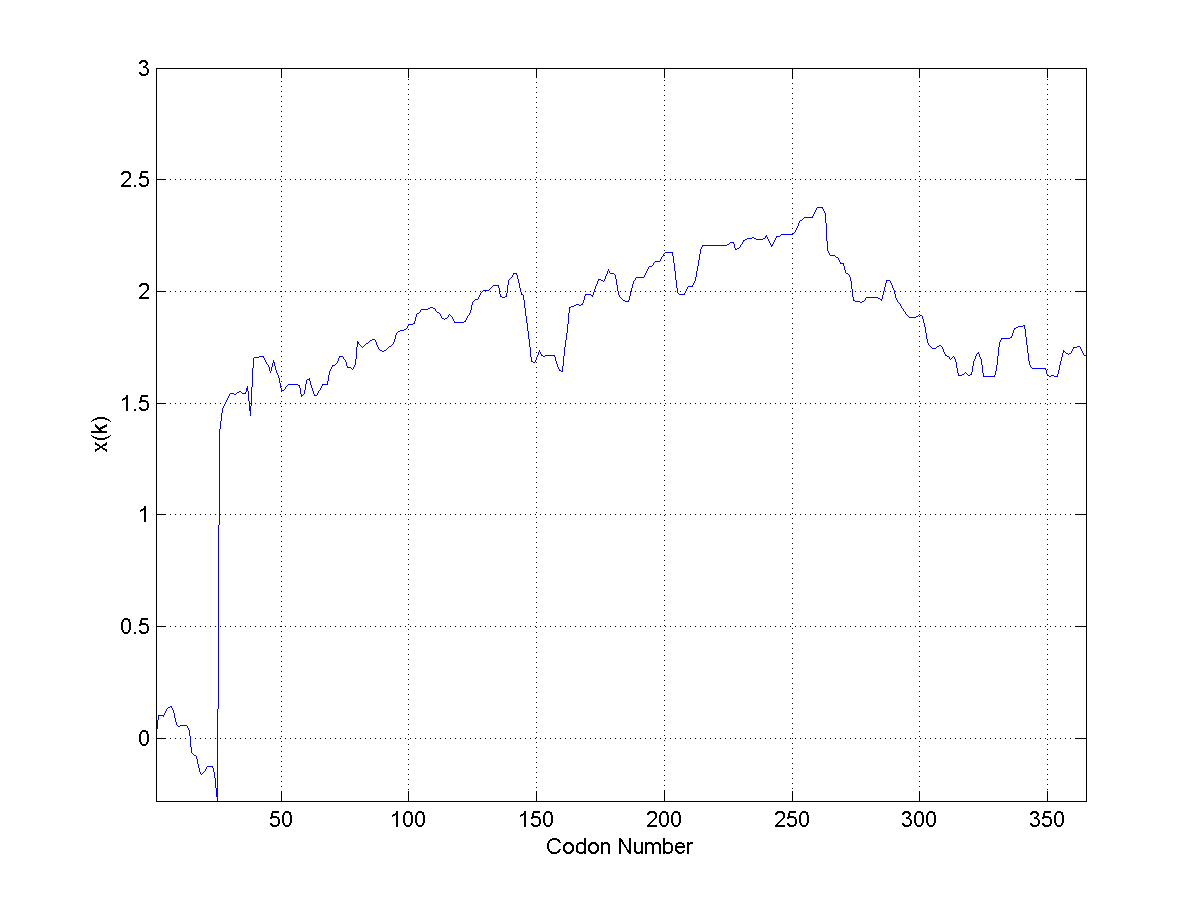
\includegraphics[width=0.4\textwidth]{prfB/disp}
  }
  \subfloat[Sensitivity plot]{
    \label{prfB:sens:sub}
    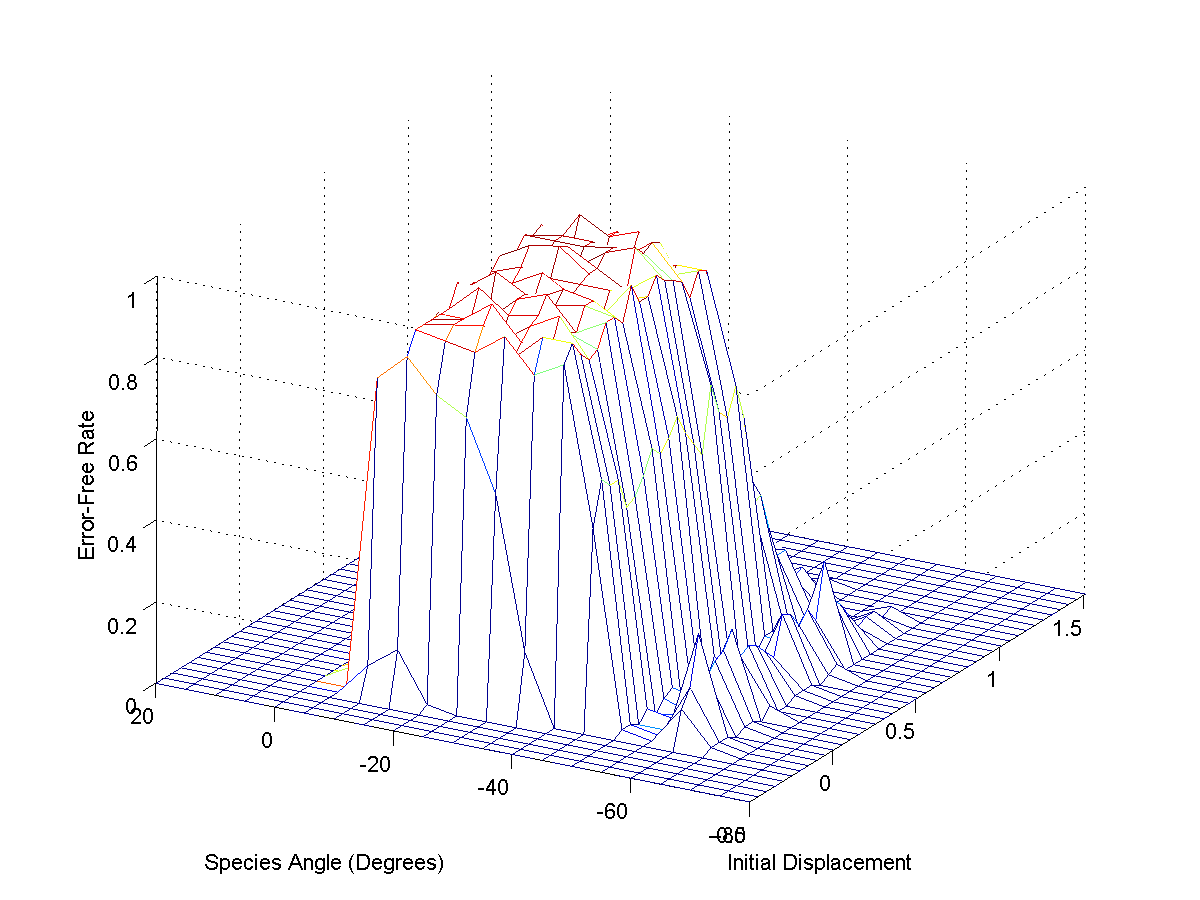
\includegraphics[width=0.5\textwidth]{prfB/sensitivity}
  }
\end{cfigure}

The gene \prfB, as mentioned, is known
to have a programmed frameshift at the 25$^{\textrm{th}}$ codon.
\autoref{prfB:disp:sub} shows its displacement plot,
again with a distinctive jump at codon 25.
\footnote{Note that the polar plot is the the same as \autoref{prfB:polar:sub}.
The new model does not alter the polar plot or the free energy calculations.}

Notably, the displacement plot does not reach $x=2$ over the span of
one codon, as the previous deterministic model predicted.  Rather, due to randomness, the
ribosome stabilizes the codon of the $+1$ frame in the A-site before actually reaching
a displacement of exactly 2.  The propensity to approach $x=2$,
however, concurs with experimental evidence indicating the ribosome
stays in frame after the \prfB\ frameshift to produce full-length RF2.
  
\autoref{prfB:sens:sub} shows the error-free rate of \prfB\ as a function
of species angle and initial displacement and demonstrates the
robustness of our model (\autoref{section:discussion}).

\begin{wrapfigure}{R}{0.5\textwidth}
  \caption{Comparison of experimental yield and error-free rate, 500 iterations}
  \label{weissboxplot}
  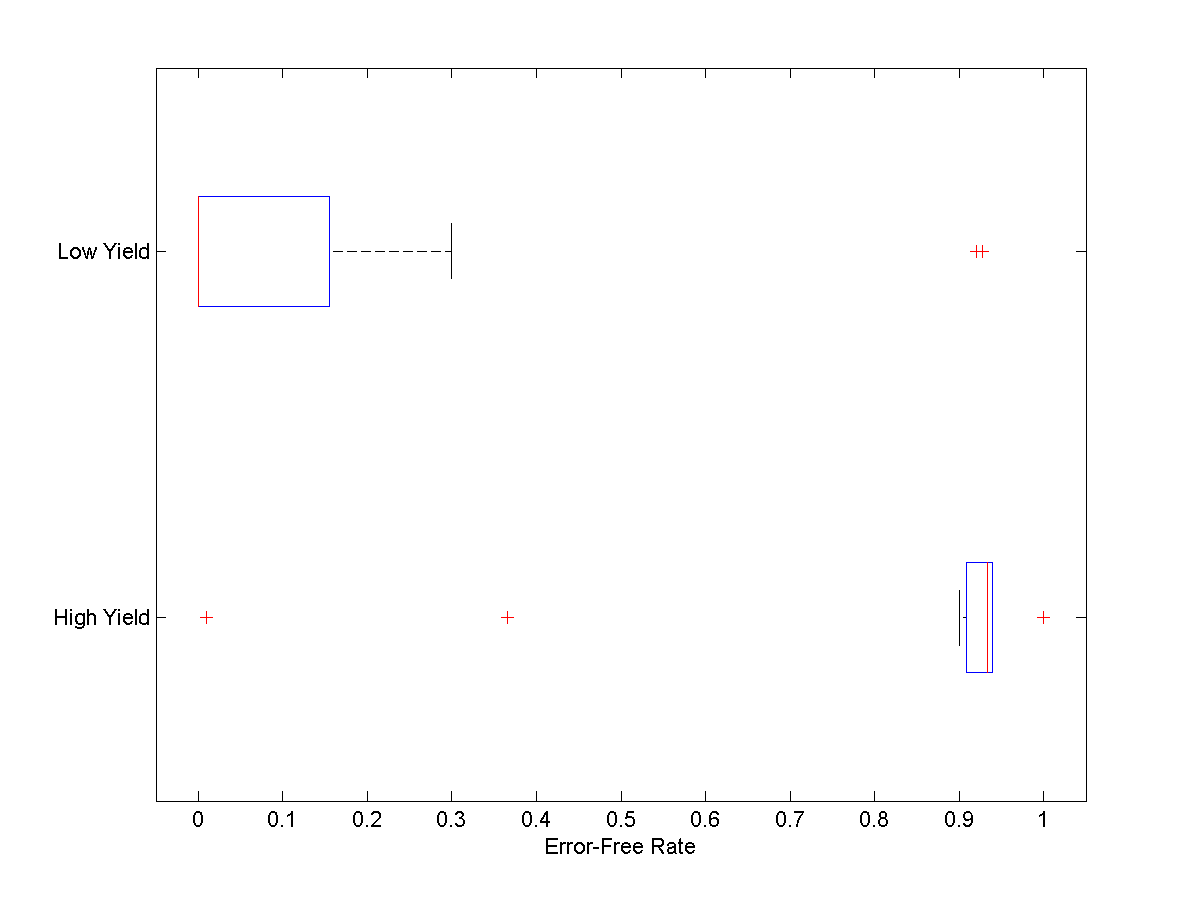
\includegraphics[width=0.5\textwidth]{histograms/weissbox}
\end{wrapfigure}

Next, we used our computational model to determine whether a correlation exists between 
error-free rate and the yield of a reporter protein, $\beta$-galactosidase (\bgals).  
\citet{weiss87} investigated elements of the mRNA sequence that could change the frequency 
of frameshifting.  The frameshift site of \prfB\ was fused to the encoding sequence for 
\bgals\ so that \bgals\ activity was dependent on the frameshift occurring, 
thus serving as an indirect measure of frameshift frequency.  

Our metric, error-free rate, showed some ability to divide Weiss'’s 35 constructs into 
two general categories: those with \bgals\ activity over 1650 whole-cell units and those with a 
lower activity.  This number is in relation to the original, unmodified \prfB\ sequence, 
which exhibited an activity of 6600 units.  These computations results suggest that 
error-free rate could be used to predict protein yield, although it lacks resolution.

Notably, \citeauthor{weiss87} did not maintain the amino acid structure of the polypeptides.  
This discrepancy may impact protein folding and half-life.  Although \citeauthor{weiss87} 
present no evidence evaluating this idea, such a phenomenon would confound the interpretation 
of \bgals\ activity as a measure of frameshift frequency.

\subsection{\ecoli\ Genes}
\begin{cfigure}
  \caption{Investigating a large sample of \ecoli\ genes}
  \subfloat[Displacement deviations]{
    \label{ecoli:hist}
    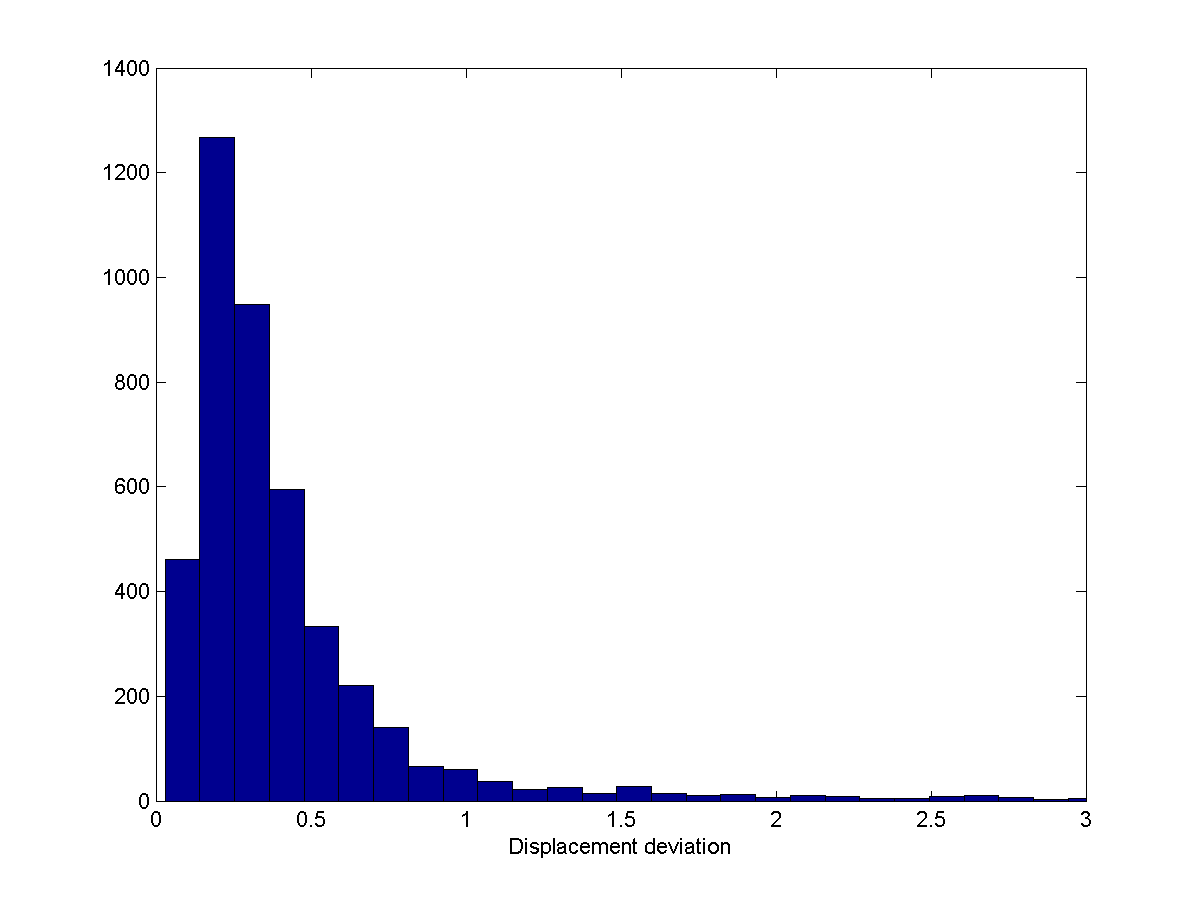
\includegraphics[width=0.4\textwidth]{histograms/everything}
  }
  \quad
  \subfloat[Comparison to ribosomal proteins]{
    \label{ribosomal:comp}
    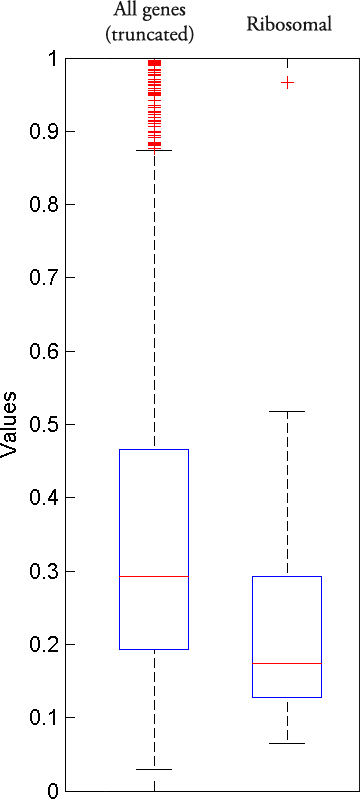
\includegraphics[width=0.5\textwidth]{histograms/ribosomal}
  }
\end{cfigure}

\autoref{ecoli:hist}\footnote{We truncate the histogram at three, excluding
  the outliers and less than 1\% of the sample.} is a histogram of the
deviation yields of 4364 genes of \ecoli, encompassing over 80\% of the entire
genome.  As predicted, 93.45\% of the genes that had deviations in the 0
to 1 interval, agreeing with the theory of natural efficiency.  The
average displacement deviation for these \ecoli\ genes is 0.4425 ($\sigma = 0.1537$), 
running 500 iterations per gene.

\subsection{Ribosomal Proteins}
\label{section:riboproteins}
To further test our idea that genes that translate efficiently should exhibit
low displacement deviations, we tested our model on ribosomal proteins, which
are known to be expressed at especially high levels.
The displacement deviation from $x=0$ for ribosomal proteins
is on average 0.2708 ($\sigma = 0.0884$) in comparison to the average of 0.4425 for our
large sample of \ecoli\ genes, which is significantly higher with a $p$-value of
0.0109 when performing a two-sample $t$ test on the means.

\subsection{Bovine Growth Hormone}
\label{section:bgh}

\begin{cfigure}
  \footnotesize
  \caption{Data for bGH}
  \subfloat[Displacement plot]{
    \label{bgh:disp}
    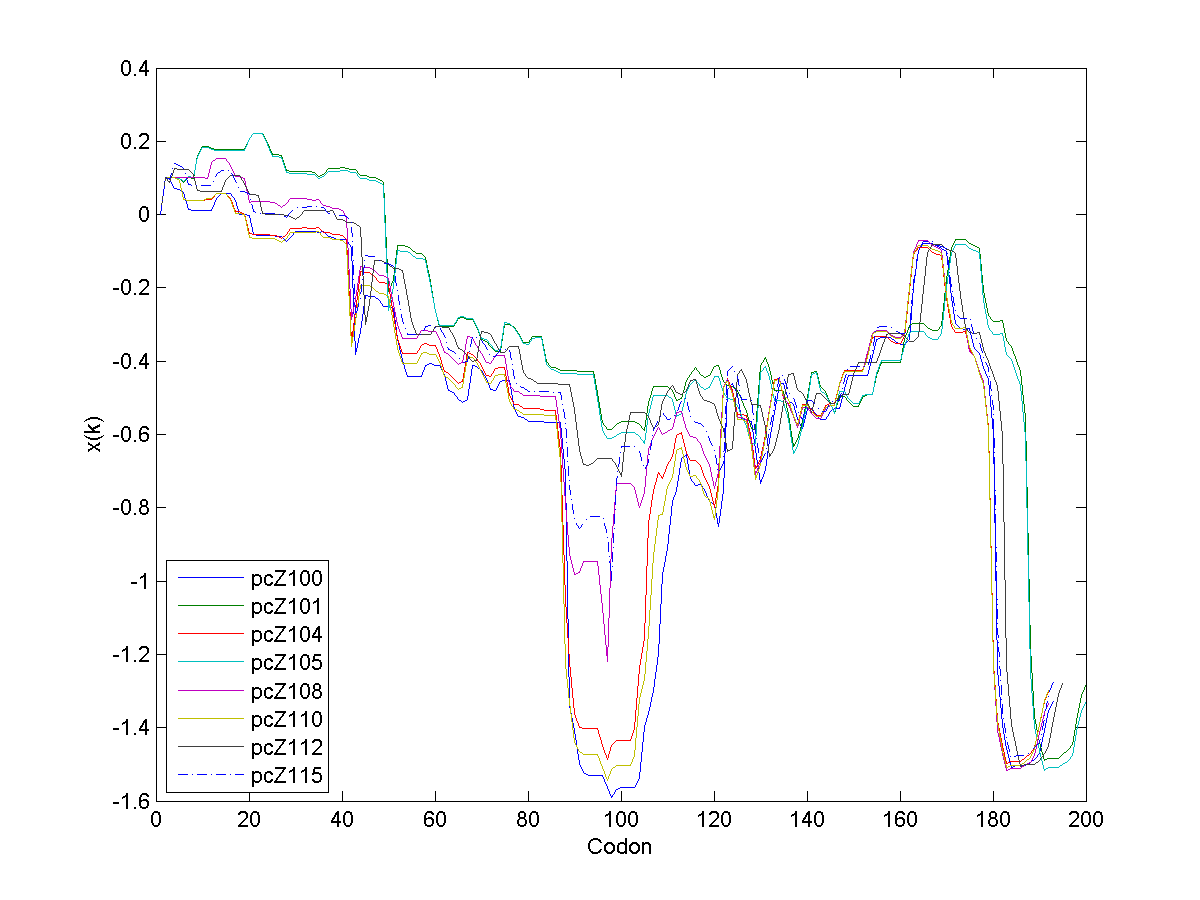
\includegraphics[width=0.45\textwidth]{bgh/all}
  }
  \subfloat[Deviations with Sample Size~500]{
    \label{bgh:deviation}
    \begin{tabular}{lccc}
  \toprule
  \textbf{Sequence} & $d$ & $\sigma(d)$ & Yield (\% bGH)\\
  \midrule
  pCZ101 & 0.5146 & 0.03313 & 30 \\
  pCZ105 & 0.5139 & 0.04181 & 34\\
  pCZ112 & 0.6612 & 0.03633 & 33\\
  pCZ115 & 0.6721 & 0.03792 & 32\\
  \midrule
  pCZ100 & 0.7107 & 0.01715 & $<$ 0.5\\
  pCZ104 & 0.7162 & 0.01433 & $<$ 0.5\\
  pCZ108 & 0.5912 & 0.05976 & 1.7\\
  pCZ110 & 0.7026 & 0.01966 & $<$ 0.5\\
  \bottomrule
\end{tabular}

  }
\end{cfigure}

We investigated the concept of displacement deviation as a predictive parameter
for experimental yield using published expression data~\cite{schoner:bgh} for bovine growth hormone (bGH).
The focus of this research was to modify the bGH mRNA sequence to optimize
yield of the protein in an \ecoli\ expression system.

\citet{schoner:bgh} created a number of constructs, primarily modifying the initial codons of a
bovine growth hormone sequence.  The research found sequences pcZ101,
pcZ105, pcZ112, and pcZ115, to have particularly high protein yields
in comparison to the four other sequences. We found these four sequences  to have the least
displacement deviation from $x = 0$
(\autoref{bgh:deviation}). \autoref{bgh:disp} shows the displacement
plots of all the bGH sequences on the same set of axes. 
Despite running the genetic algorithm to improve tRNA availability vectors, pcZ108 remains an
outlier because \citeauthor{schoner:bgh} reported low protein
yield whereas our model reports low deviation, indicative of 
high protein yield.

Once again, it must be noted that, like \citeauthor{weiss87}, \citeauthor{schoner:bgh}
did not maintain the amino acid sequence while modifying the nucleotide sequences of the bGH constructs.
The sequence pcZ108 encodes a different amino acid sequences than the other constructs.
The lower translational efficiency may be attributed to the interaction
of the primary structure with the ribosome and not to any signal encoded
in the mRNA.

\subsection{An Artificial Frameshifter}
\label{section:linker}
\begin{wrapfigure}{R}{0.5\textwidth}
  \centering
  \caption{Artificial linker sequence sensitivity plot}
  \label{linker:sens}
  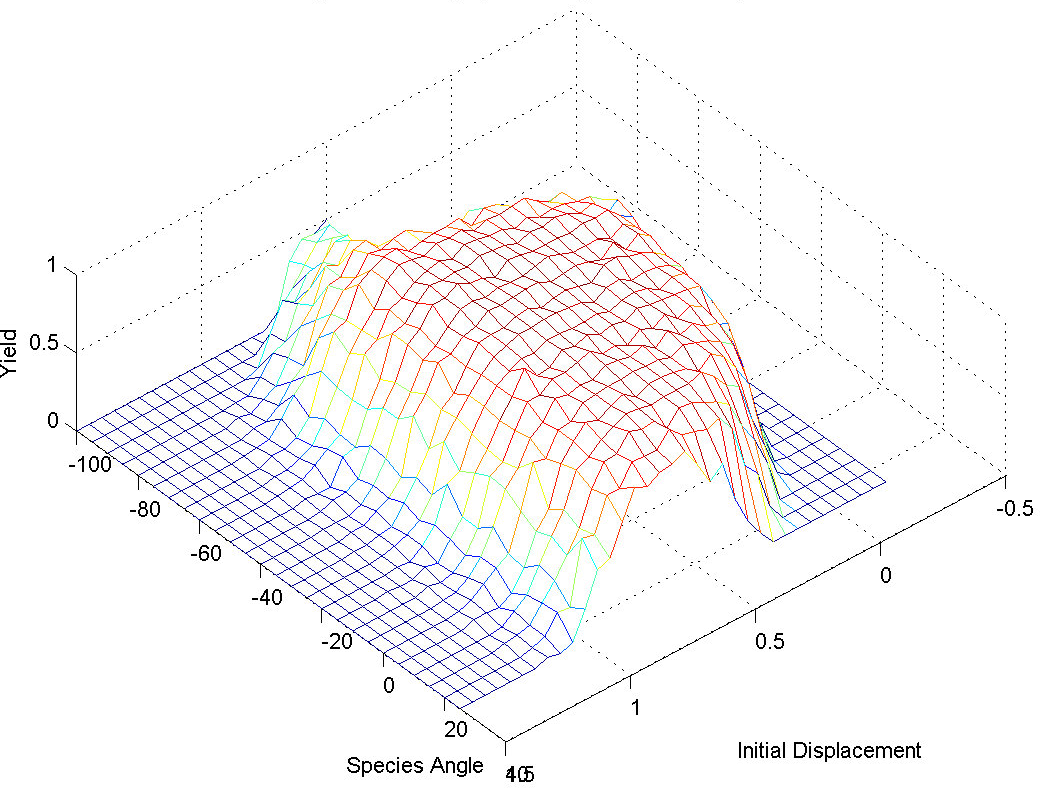
\includegraphics[width=0.45\textwidth]{linker/sensitivity}
\end{wrapfigure}

\begin{cfigure}
  \caption{Artificial linker sequence with a 12-base leader sequence
    in brackets}
  \label{linker}
  \begin{verbatim}
    [aga aau cag acc] aug gag gcu ggc acc agg ggg uac agu  u  aag caa acg
  \end{verbatim}
\end{cfigure}

To verify our model's predictive ability, we focused on its ability to
predict programmed frameshifts. We designed a sixteen-codon sequence
with such a frameshift (\autoref{linker}) in \ecoli\ into
the \textsc{aag} frame after crossing the sole uracil.  Figure~\ref{linker:sens}
shows the error-free rate of the linker sequence as a function of species
angle and initial displacement, which is as robust as \prfB\ (\autoref{prfB:sens:sub}).

Next, we performed a BLAST search, which found no similar sequences in 
\ecoli\ or known to possess a frameshift. We found only 30 matches, all 
of which meet neither of the criteria. Then, working with molecular 
biologists, we helped design a strategy to use a bifunctional fusion 
protein containing beta-galactosidase (\bgals) and \xylE, with \xylE\ in 
a +1 reading frame. \bgals\ levels are quantified from the colorless 
reagent nitrophenol-galactosidase that, when cleaved by \bgals, yields 
nitrophenol, which has a yellow color; \xylE\ cleaves the carbon ring 
of catechol.  These two proteins and the proposed linker sequence join 
to form a fusion protein.  Research indicates that even in this fused 
protein, both \bgals\ and \xylE\ should retain their functionalities.
As such, if the frameshift were to occur, one should observe high 
levels of both nitrophenol and catechol cleavage products.

We are working with a graduate student with molecular biology expertise 
who has constructed a plasmid made of an ampicillin gene, the \emph{lacZ} 
operon, our linker sequence, and the catechol enzyme gene \xylE\ in order 
to measure the frameshift efficiency of our linker sequence in addition 
to other control groups. The experiment is a work in progress.

\section{Discussion}
\label{section:discussion}

The purpose of our studies was to extend and improve the deterministic
model of \citeauthor{lalit:mechanics}, which gave a mechanistic
perspective of ribosomal movement during translation and a genetic
signal approach to translating mRNA sequnences. It incorporated a
number of parameters including
codon bias~\cite{ikemura} and rare codon usage~\cite{kane95} known to
affect translation. The model also could predict frameshift locations
in the sequence, of value in sequence annotation i.e. frameshift identification.
Our studies extended this predictive power to 
computationally predicting translational efficiency.

The deterministic structure limited the \cite{lalit:mechanics} model.
We restructured it into a stochastic process where cellular
environment conditions can affect translation. In essence, the
stochastic model paints a more realistic picture of the ribosome, a
machine that makes choices nondeterministically due to noise from the
cell environment.

In addition to the stochastic version, we also developed two metrics:
error-free rate (\autoref{section:efr}) and displacement deviation
(\autoref{section:deviation}). Error-free rate
provides a measure of an mRNA sequence's propensity to frameshift by
measuring reading frame change frequency.  Notably, replicating the experiments
of \citet{weiss87} shows it can roughly separate sequences into
those with high and low frameshift frequencies. However, the
resolution provided by the model is not clear and we must turn to
displacement deviation in these cases.

Displacement deviation (\autoref{section:deviation}),
when run upon a large sample of \ecoli\ genes known to be translationally efficient,
correlated with over 90\% of the  experimental data, predicting
these genes to be efficient.  Moreover, it predicts that ribosomal proteins should
be more efficient than average.  Displacement deviations for eight bGH
sequences~\cite{schoner:bgh} also roughly correlates with further
experimental data; one sequence proved to be an outlier.

Since the model is preliminary, we must note these outliers.  In the
bGH, \citeauthor{schoner:bgh} experimentally determined pcZ108 to be
of low yield, but the model computationally predicts high yield.
Likewise, in the set of constructs used by \citet{weiss87}, where one
set gave of low yield, the model again predicted differently.  One
possible explanation of these discrepancies relates to the chemical
structures of the mRNA sequences and the polypeptides they
encode.  In both cases, \citeauthor{weiss87} and
\citeauthor{schoner:bgh} did not maintain the amino
acid structure while designing the sequences. If a protein-ribosome
interaction or post-translational instability resulted from these
changes, then such a change significantly impacts protein yield, an
indirect measure of translation. However, these effects on
translational efficiency are beyond the scope of our model.

We also plan to explore parameter estimation in future studies.
Analysis of \prfB\ and the
proposed linker sequence suggest our model is robust with respect to species angle
and initial displacement, but proper estimation of tRNA availability
poses a problem. \citet{lalit:mechanics} based these values solely on 
codon usage, but research~\cite{phelps} also suggests that tRNA shape
also determintes overall availability as it is known to affect
frameshift frequency. The
genetic algorithm (\autoref{section:parameters}) we created thus
provides an initial method for a coarse estimation. However, we did
not extensively investigate this idea and thus we limited the
deviation values computed by \citeauthor{lalit:mechanics}.

Currently, our model predicts translational efficiency with some
accuracy and can distinguish between high and low yield sequences. We
need more experimental verification such as our linker sequence
(\autoref{section:linker}), currently in progress, we will adjust the
model to increase its predictive and resolving power and consequently
its importance in the field of genetics.

\section{Conclusion}
\label{section:conclusion}

In this paper, we presented a means to predict translational
efficiency.  More research is needed to accrue experimental data, incorporate
the idea of chemical interactions inherent in ribosomal translation, and
improve parameter estimates, especially those of tRNA availability
values. Despite these
shortcomings, our model's ability to discern between efficient and
non-efficient sequences provides shows tentative promise in applications
in the field of recombinant biotechnology, providing
a computational method of using \ecoli\ as an expression system
for commercial proteins.

\phantomsection
\addcontentsline{toc}{section}{References}
\begin{singlespace} \bibliography{wizards} \end{singlespace}
\end{document}

% This is for ispell. Do not delete. --Hao
% LocalWords:  abcd abc bcd sp pcZ riboproteins disp aag guu efr ikemura jbsb
% LocalWords:  kane sd xray starmer aa TAV uga NCBI's Genbank lacZ hui UAA
% LocalWords:  Ecogene schoner kozak
